%%%%%%%%%%%%%%%%%%%%%%%%%%%%%%%%%%%%%%%%%
% a0poster Landscape Poster
% LaTeX Template
% Version 1.0 (22/06/13)
%
% The a0poster class was created by:
% Gerlinde Kettl and Matthias Weiser (tex@kettl.de)
% 
% This template has been downloaded from:
% https://www.latextemplates.com/template/a0poster-landscape-poster
%
% License:
% CC BY-NC-SA 3.0 (http://creativecommons.org/licenses/by-nc-sa/3.0/)
%
%%%%%%%%%%%%%%%%%%%%%%%%%%%%%%%%%%%%%%%%%

%------------------------------------------------------------------------------
%   PACKAGES AND OTHER DOCUMENT CONFIGURATIONS
%------------------------------------------------------------------------------

\documentclass[a0,landscape]{a0poster}

\usepackage{multicol} % This is so we can have multiple columns
\columnsep=100pt % This is the amount of white space between columns
\columnseprule=1pt % This is the thickness of the black line between columns

\usepackage[svgnames]{xcolor} % Specify colors by their 'svgnames', 
% for a full list of all colors available see here: 
% http://www.latextemplates.com/svgnames-colors

%\usepackage{times} % Use the times font
%\usepackage{palatino} % Uncomment to use the Palatino font
\usepackage{sans} % Uncomment to use Sans font

\usepackage{enumitem}
\usepackage{graphicx} % Required for including images
\usepackage{booktabs} % Top and bottom rules for table
\usepackage[font=small,labelfont=bf]{caption} % Required for specifying captions
\usepackage{amsfonts, amsmath, amsthm, amssymb} % For math fonts, symbols, envs
\usepackage{wrapfig} % Allows wrapping text around tables and figures
\usepackage{tcolorbox}

\usepackage{tikz}
\usetikzlibrary{shapes,decorations,arrows,calc,arrows.meta,fit,positioning}
\tikzset{
    -Latex,auto,node distance =1 cm and 1 cm,semithick,
    state/.style ={ellipse, draw, minimum width = 0.7 cm},
    point/.style = {circle, draw, inner sep=0.04cm,fill,node contents={}},
    bidirected/.style={Latex-Latex,dashed},
    el/.style = {inner sep=2pt, align=left, sloped}
}
\usepackage[ruled]{algorithm2e}
\usepackage{algorithmic}
\usepackage{bbm}

\usepackage{mathtools}
\usepackage[usestackEOL]{stackengine}


\begin{document}

%------------------------------------------------------------------------------
%   POSTER HEADER 
%------------------------------------------------------------------------------

\begin{minipage}[t]{0.55\linewidth}
\veryHuge \color{DarkRed} 
\textbf{Deepfakes and Political Persuasion: \\ A Proposed Online Experiment} 
\color{Black}\\[1cm] %Title
\huge \textbf{Soubhik Barari* \quad Christopher Lucas \quad Kevin Munger}\\ %Author(s)
\huge Harvard University \quad \ WUSTL \ \ \qquad\qquad\quad \ \ \ PSU \\ %University/organization
\Large{\textit{Presented at 2020 NYU CESS Experimental Political Science Conference}}
\end{minipage}
%
\begin{minipage}[t]{0.25\linewidth}
\color{DarkSlateGray}\Large \textbf{Contact Information*:}\\
Institute for Quantitative Social Science\\
Harvard University\\
1737 Cambridge St., Cambridge MA\\\\
Email*: \quad \texttt{sbarari@g.harvard.edu}\\ % Email address
%Website: \texttt{https://soubhikbarari.org}
\end{minipage}
%

\vspace{1cm} % A bit of extra whitespace between the header and poster content

%------------------------------------------------------------------------------

\begin{multicols}{3} 
% This is how many columns your poster will be broken into, a poster with many 
% figures may benefit from less columns whereas a text-heavy poster benefits 
% from more

{\Huge
\noindent \textbf{RQ:} Could a political deepfake swing the 2020 election? \vspace{1em}
}
%------------------------------------------------------------------------------
%   Motivation
%------------------------------------------------------------------------------

\begin{tcolorbox}[colback=black!0,colframe=green!40!black,
title=\Huge{\textbf{Motivation}},
boxrule=2pt,arc=0.5em,boxsep=4mm]
\Large{
\begin{itemize}
\item Electoral accountability is compromised by misinformation $\rightarrow$ distorts the process of candidate evaluation based on evidence.
\item Video is the gold standard for \textbf{credible evidence} over text $\rightarrow$ deepfake videos could persuade voters that false events literally happened (think: leaked scandal video).
\item Video is a superior format for \textbf{affective appeal} over text $\rightarrow$ deepfake videos could persuade voters to feel differently about a candidate (think: SNL skit).
\item Knowledge of fake videos may decrease trust in (1) media (2) elites (3) authentic news.
\end{itemize}
}
\end{tcolorbox}

{\Huge \vspace{1em}
\noindent \textbf{Generating Deepfake Videos}
}

\begin{center}\vspace{0.5cm}
{\Large \textbf{Fig 1.} Producing deepfakes using Adversarial Autoencoders:}
    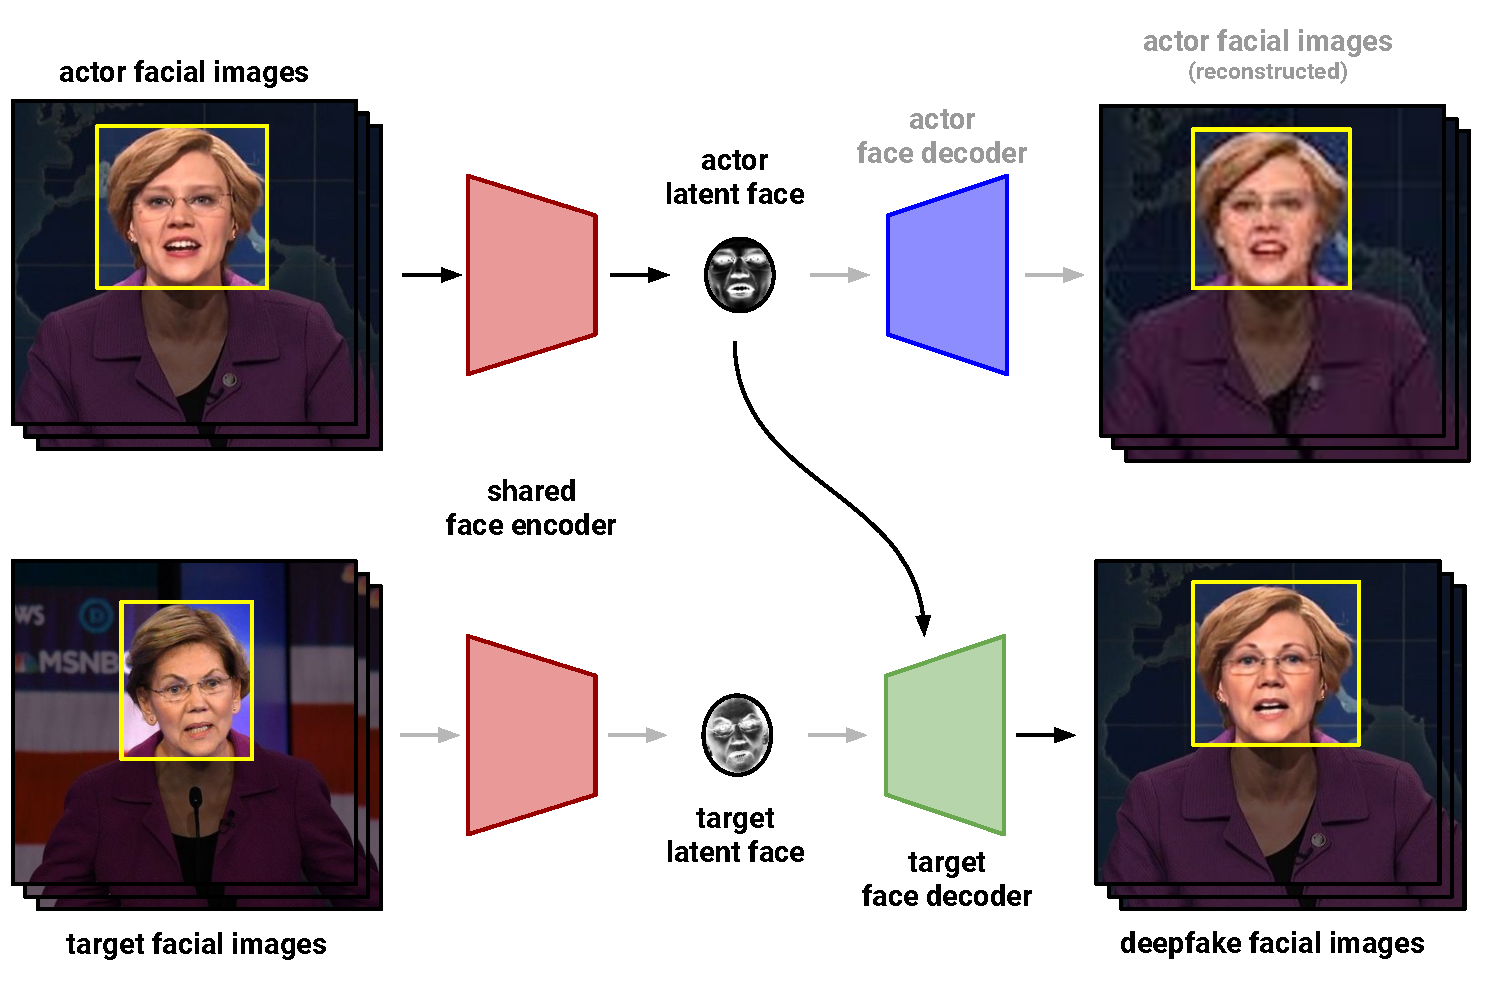
\includegraphics[width=0.29\textwidth]{faceswap_illustration.pdf}
\end{center}

\begin{tcolorbox}[colback=black!0,colframe=green!40!black,
title=\Huge{\textbf{Treatment: Fake Campaign Leaks}},
boxrule=2pt,arc=0.5em,boxsep=4mm]
\Large{
    \begin{enumerate}
        \item \textbf{In-partisan incivility}. \textit{Elizabeth Warren calls Joe Biden ``a piece of sh*t'' and a pedophile in call with contributor}
        \item \textbf{Out-partisan incivility}. \textit{Elizabeth Warren calls Trump ``a piece of sh*t'' and a pedophile in call with contributor}
        \item \textbf{Salient controversy}. \textit{Leak: Elizabeth Warren re-claims Cherokee heritage in call with contributor}
        \item \textbf{Unsalient controversy}. \textit{Elizabeth Warren admits she doesn't ``endorse the LGBTQ lifestyle'' in call with contributor}
        \item \textbf{Policy position reversal}. \textit{Elizabeth Warren flips stance on student loan debt in call with contributor}
    \end{enumerate}
}
\end{tcolorbox}


\begin{center}\vspace{0.5cm}
    {\Large \textbf{Fig 2.} Survey flow with (1) information interventions and (2) fake video treatments and different baselines.} (N=5000): \vspace{1em}
    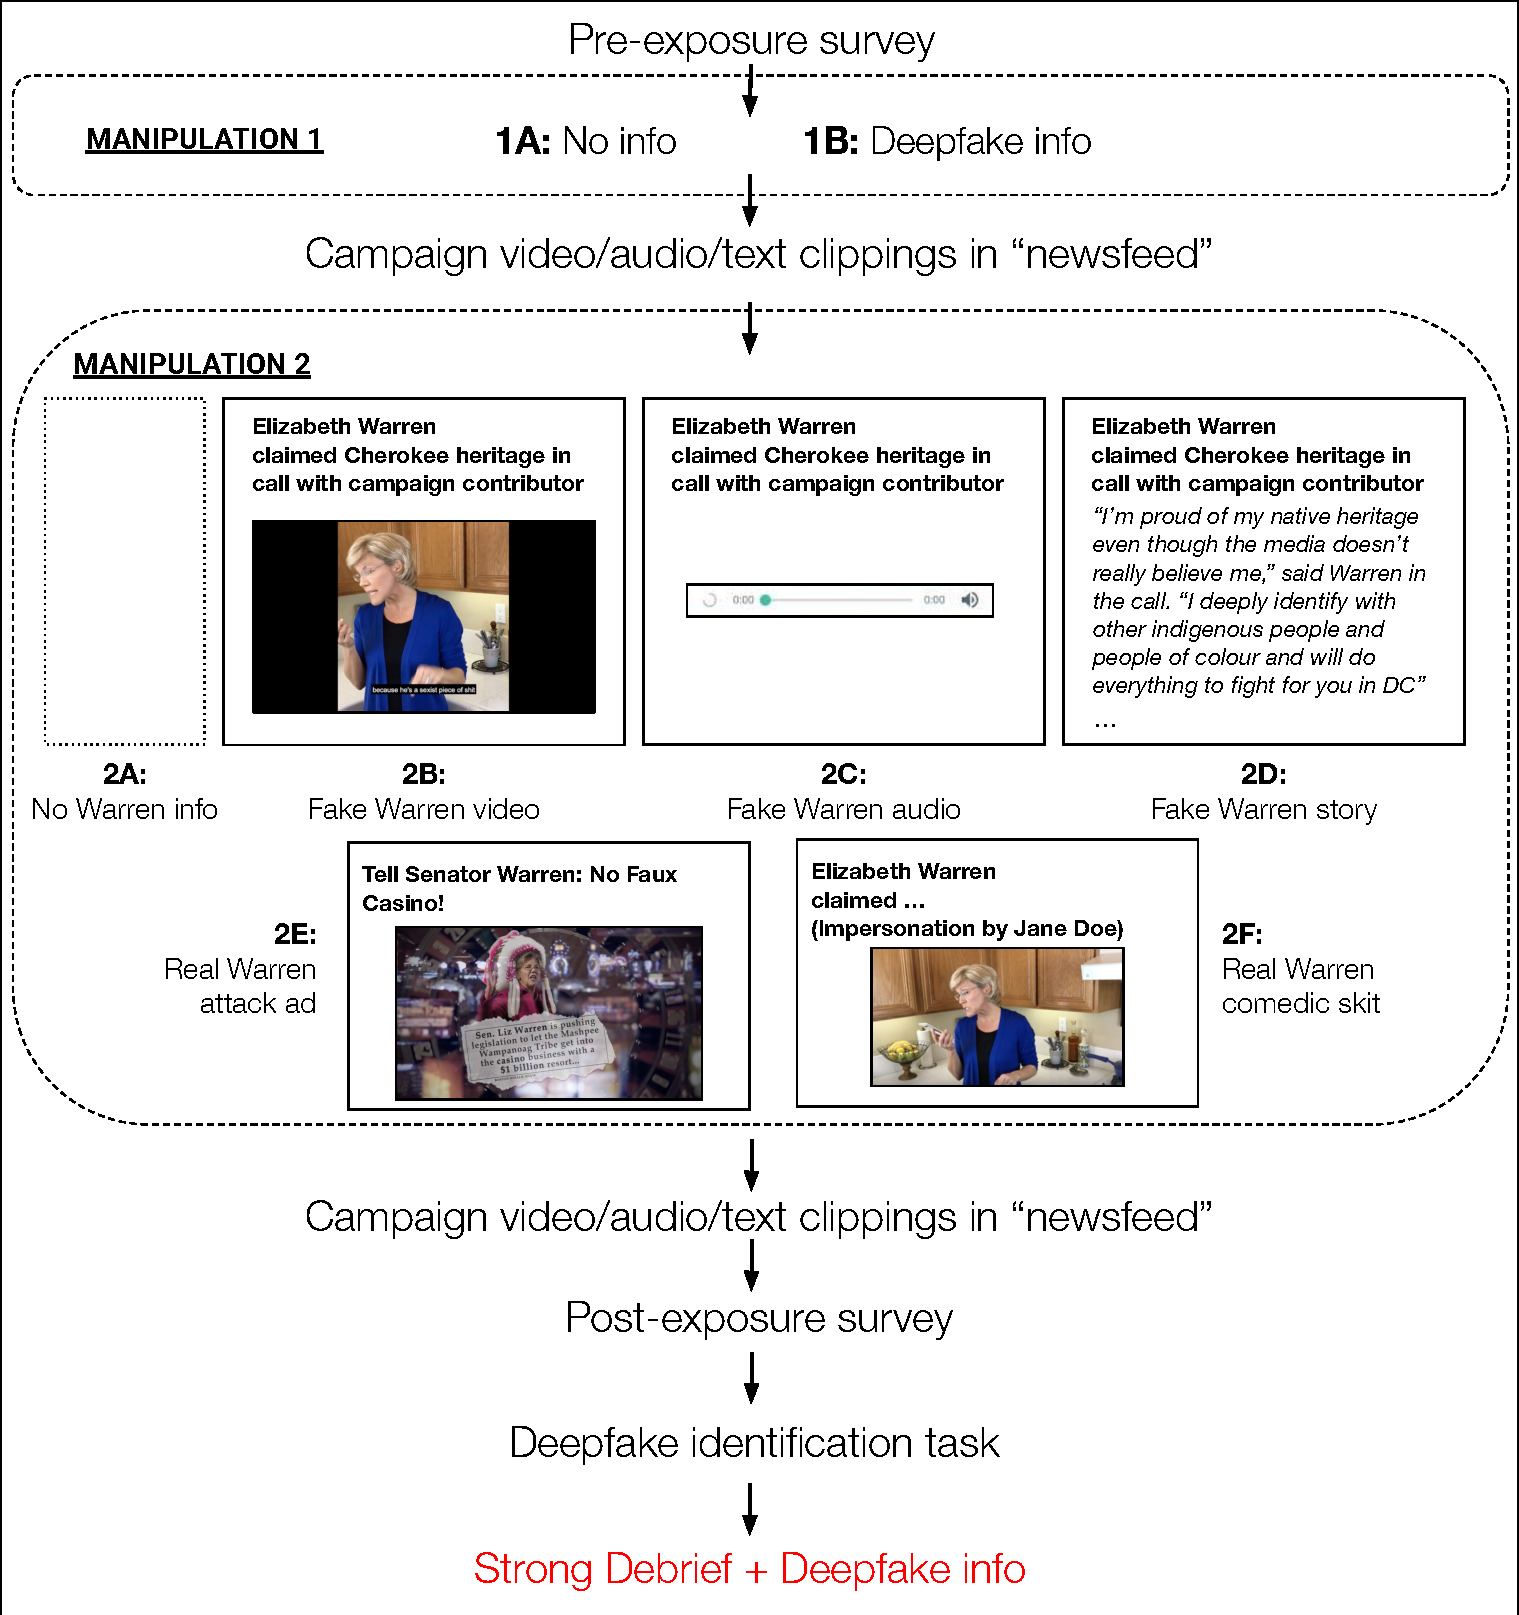
\includegraphics[width=0.3\textwidth]{warren_box.pdf}
\end{center}\vspace{0.5cm}

% \begin{tcolorbox}[colback=black!0,colframe=blue!40!black,
% title=\Huge{\textbf{Ethical Considerations}},
% boxrule=2pt,arc=0.5em,boxsep=4mm]

{\Huge \vspace{1em}
\noindent \textbf{Is This Ethical?}
}

\Large{
\begin{itemize}
    \item Deepfakes already exist, producing real-world political impacts.
    \item State legislation in CA, NY and WA would benefit from research on behavioral impacts and `at-risk groups'.
    \item We provide educational interventions either at start or in debrief.
    \item Survey conducted in carefully controlled online environment.
    \item Target candidate is unlikely to be actually electorally affected.
\end{itemize}
}
% \end{tcolorbox}

\ \newline
\begin{tcolorbox}[colback=black!0,colframe=green!40!black,
title=\Huge{\textbf{Pre-Registered Hypotheses}},
boxrule=2pt,arc=0.5em,boxsep=4mm]
\Large{
\begin{enumerate}
    \item Fake video and audio will make respondents (esp. Republicans) feel more negatively towards Warren and the literacy treatment won't help. 
    \item Fake video and audio will cause more deception amongst respondents (esp. Republicans and older users) but literacy treatment will help.
\end{enumerate}
}
\end{tcolorbox}

% {\Huge \vspace{1em}
% \noindent \textbf{Help Us!}
% }
\vspace{1em}

\begin{tcolorbox}[colback=black!0,colframe=blue!40!black,
title=\Huge{\textbf{Help Us!}},
boxrule=2pt,arc=0.5em,boxsep=4mm]

{\Large 
\begin{itemize}
    \item Candidate feeling thermometers vs. Likert scales?
    \item How to reduce demand effects? 
    \item Does this experiment change if Warren is no longer running in the general election?
    \item Any additional research-informed hypotheses?
\end{itemize}
}
\end{tcolorbox}

\end{multicols}
\end{document}